Un péndulo de 1 kg se balancea del punto A, de altura y$_A$=10 cm, al punto B, de altura y$_B$=7 cm. Las alturas son relativas a la altura más baja. ¿Cuál es el cambio en la energía potencial gravitacional de A a B?

\begin{minipage}{0.68\textwidth}
    \begin{solutionbox}{5.8cm}
        \begin{multicols}{2}
            Datos:

            E$_p$ = ?

            \[
                \begin{array}{rl}
                    \Delta y & = y_B - y_A                       \\
                             & = 0.07 \text{ m} - 0.10 \text{ m} \\
                             & = -0.03 \text{ m}
                \end{array}
            \]
            g= 9.8 m/s$^2$

            m = 1 kg

            \vspace{2cm}

            La energía potencial es:
            \[E_p=mg\Delta y\]


            Sustituyendo nuestros datos en la fórmula:
            \[
                \begin{array}{rl}
                    E_p & = (1 \text{ kg})(9.8 \text{ m/s$^2$})(-0.03 \text{ m}) \\[1em]
                        & =-0.29 \text{ J }
                \end{array}
            \]

        \end{multicols}
        \begin{center}El cambio en la energía potencial del carrito del punto A al B es de -0.29 J.\end{center}
    \end{solutionbox}
\end{minipage}\hfill
\begin{minipage}{0.25\textwidth}
    \begin{figure}[H]
        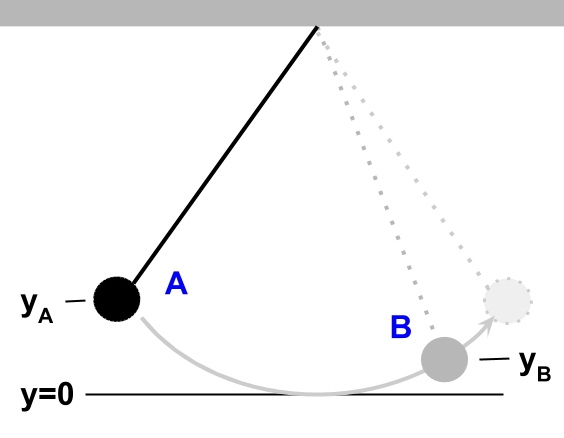
\includegraphics[width=\linewidth]{../images/4a243ab80f29a94e88f7c5425b2c9bfe54cd78a6}
    \end{figure}
\end{minipage}
